% Source: tex/chapters/ch05/06_テスト技法.tex
\subsubsection{構造ベーステスト技法}
構造ベース技法は、コードや設計の内部構造を情報源としてテストケースを選ぶ。ホワイトボックス技法とも呼ばれる。文カバレッジ、分岐カバレッジ、経路カバレッジ、循環的複雑度などが関係する。

\paragraph{制御フローテスト}
制御フローテストは、文、分岐、判定、条件、条件組合せ、経路を対象に、どの部分を実行したかを確認する。最も強い基準の一つはすべての入口から出口までの経路を通す経路テストであるが、ループがあると現実的でないため、文カバレッジ、分岐カバレッジ、条件判定カバレッジなどの基準が使われる。

\paragraph{データフローテスト}
データフローテストは、変数の定義、使用、未定義化に注目する。ある変数が定義された後、どの経路でどの使用に届くかを確認する。定義と使用の組合せを扱うため、データに関する隠れた欠陥を見つけやすい。

\paragraph{構造ベース技法の参照モデル}
構造ベース技法では、制御フローグラフがよく使われる。ノードは文や文列を表し、辺は制御の移動を表す。この図に基づいて、どの文、分岐、経路を通したかを可視化できる。

\begin{figure}[htbp]
\centering
\IfFileExists{assets/generated_figures/ch05/fig-ch05-09.png}{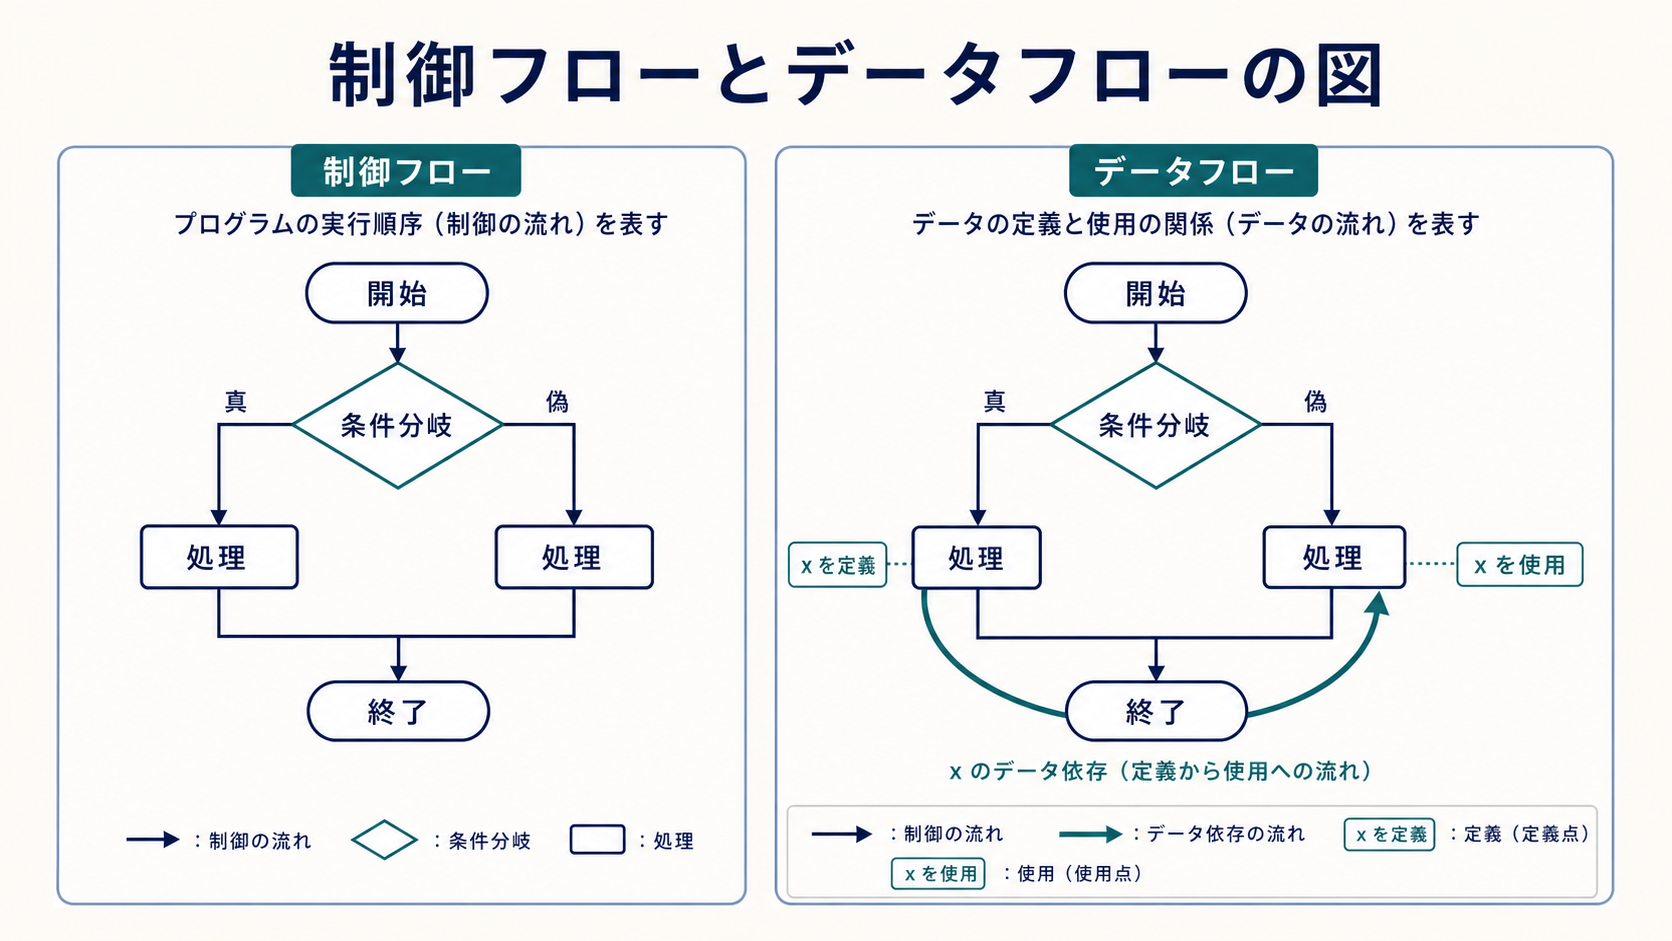
\includegraphics[width=0.96\linewidth]{assets/generated_figures/ch05/fig-ch05-09.png}}{\fbox{\parbox[c][48mm][c]{0.9\linewidth}{\centering 画像生成待ち\\制御フローとデータフローの図}}}
\caption{制御フローとデータフローの図}
\label{fig:ch05-09}
\end{figure}
